\section{A Customized Programming Environment}
\label{sec:environment}


The features that influence the experience of the learning programmer are not limited to the programming language she uses. 
The \emph{tools} through with the code is written, analyzed and evaluated have a paramount relevance for this experience, and therefore for the success of the programming courses.

Beginner programmers are likely to require more guidance and make more mistakes than experienced programmers.
Also, the kind of support required by experienced programmer from her development environment is different from that required by a beginner, \eg an experienced programmer might select her programming environment thinking on increasing productivity.
One very important feature a beginner requires from her programming environment is \emph{discoverability}, \ie the tools should help discover possible paths of action and gently provide feedback when the student makes a mistake, helping her to understand what was wrong and how to fix her program.
Finally, all programmers require tools that help them understand, navigate and explore their programs.

\medskip 

We decided to embed the Wollok language in an integrated programming environment, whose features are designed having in mind the specific needs of novice programmers.
In our view. the tools provided by the environment are a fundamental part of the Wollok proposal, in equal terms with the language features.

In particular, the Wollok environment provides tools focused to the following goals:
\begin{itemize}
\item To guide and ease the acual code writing.
\item To detect several of the most common mistakes done by novices, providing adequate feedback, and even to provide possible corrections when they can be computed.
\item Navigate an give different perspectives of the defined objects and classes.
\item Organize the code that is produced along the course.
\item Test and experiment with objects, both those provided by the student and those provided by Wollok.
\end{itemize}

We remark that several of the tools that the Wollok environment provides are common, in exact or approximate form, to those provided by mainstream industrial IDEs like e.g. Eclipse, Visual Studio or the Idea series. In this way, we aim to make both the programming experience more appealing to the students, and the transition to later courses and work environments softer; while giving adequate support to the learning process through the same tools.

\subsection{Basic guidance for writing code}
% To guide and ease the acual code writing
We have noticed that the first barrier for novices is the strictness of a programming language syntax. Frequently initial students find annoying that their program will not execute if they forget a closing brace or mispell a keyword or a variable name, in many cases even a case error stops execution or produces unexpected results.
Syntax highlighting is very helpful by providing a very fast visual feedback about a mispelled keyword.
Also, like many modern code editors, the Wollok IDE automatically creates a matching closing symbol each time the programmer types a parenthesis, square braket or braces. 
Also the IDE helps correctly indenting the code inside code portions enclosed in braces or square brakets, which both helps avoiding frustrating syntax problems and starts to induce best practices about code organization.

Other approaches have addressed this problem using block-based or visual programming tools \np{Cita a alguno}. 
While we value those ideas, we think that mainstream programming is and will continue to be text-based, therefore, non-textual programming can be useful for younger students, but at universitary level it is better to provide tools that help dealing with syntax problems rather than continue circumventing them.

At a bigger scale, Wollok admits the definition of several objects and/or classes in the same file. 
This allows the teacher to go deeper in the initial examples in playing with several objects and polymorphism, without requiring the students to struggle with imports and packages.
These concepts will arise later in the course, when students' programs increase their complexity to a level that demands for modularization (\cf \ref{sec:modularization}).
\np{¿Esto no es una característica del lenguaje?}

The Wollok IDE also has integrated a powerful \emph{code analyser} that enables for \emph{content assistance}\np{¿Está bien este nombre?}, 
\ie in certain contexts, the IDE can autocomplete an identifier name, or provide a list of possible completions if there are many (\cf Fig. \ref{fig:codeCompletion}).
This is available for all types of variables and constants and messages sent to \code{self}, \code{super} or any WKO\footnote{Current work in progress includes a type inference system that once completed should allow to add content asistance for any message send}. 
 
\begin{figure}[ht]
 \centering
 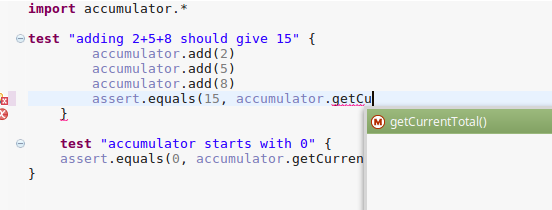
\includegraphics[scale=0.6]{images/codeCompletion.png}
 \caption{\small A list of suggestions from the Wollok IDE content assistance.}
 \label{fig:codeCompletion}
\end{figure}

% Detect errors and help fixing them
\subsection{Detecting mistakes}
To detect several of the most common mistakes done by novices, providing adequate feedback, and even to provide possible corrections when they can be computed.

  - Error indications with adequate messages. De esto daría algunos ejemplos que nos parezca piola resaltar, no sería exhaustivo.
  - Quick fixes.


The programming environment has many tools intended to help detecting mistakes.
We make special emphasis in detecting errors \emph{while} the student is writing code. \np{Acá se podría hablar más}
\emph{Syntax highlighting} helps identify the most simple mistakes by providing immediate feedback when something is not right. 
Moreover, the environment provides \emph{real-time highlights} for several kinds of mistakes (\cf \figref{check-noMethodOnThis.png}).
Finally, the environment has a (basic) \emph{type inferer} which in some cases detects more subtle mistakes.

\begin{figure}[ht]
    \centering
	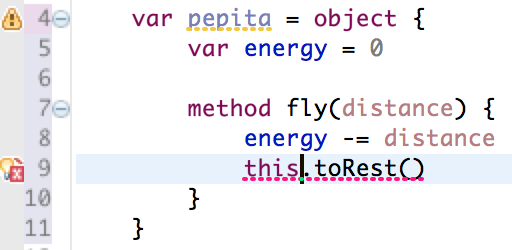
\includegraphics[scale=0.5]{images/wollok-paper-check-noMethodOnThis.png}
    \caption{Detection of an error sending a message to \emph{this} which doesn't exist}
    \label{fig:check-noMethodOnThis.png}
\end{figure}

% Este no sé cómo ponerlo, es muy crítica al smalltalk.
% 8-reducir errores frustrantes: se cancela la edicion por tener 1 solo editor de metodo por ves (poder visualizar más que un sólo método simul), evitar errores de imagenes)

This validations are organized and shown in a unified way, using a dedicated section of the user interface for their display.
All the results of the checking and the validation of the program is shown in one integrated view, it is called \emph{Problems View}, Fig. \figref{problemsview.png} shows a view of this feature. 

\begin{figure}[ht]
    \centering
	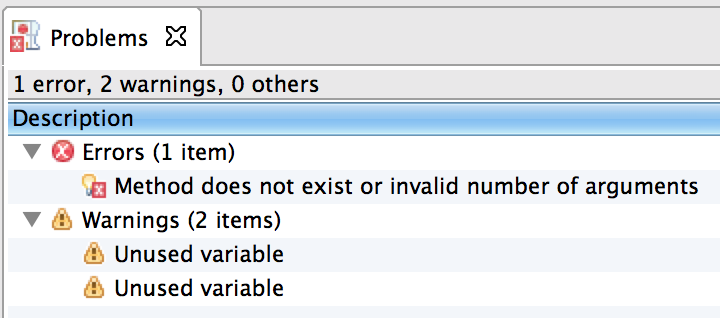
\includegraphics[scale=0.5]{images/wollok-paper-check-problemsview.png}
    \caption{Problems View: shows the different problems detected by the IDE }
    \label{fig:problemsview.png}
\end{figure}

Checks and validations are not only used to show type errors or syntax errors, 
but also to encourage some properties of the program we consider as main topics in the learning process of an OO language.
Here is a list of all the validations and checks the tool supports, and a brief reason why they are useful while teaching object oriented programming:

\begin{itemize}
  \item \textbf{Syntax Errors}: this category involves all the errors detected by the parser and the lexical analyser of the language.
  \item \textbf{Style Errors}: this category is useful to teach good practices and to start to talk about code quality, reuse and code sharing.
	\begin{itemize}
		\item \textit{Case in Names}: respecting the difference case conventions for
		names (\eg using \textit{camelCase} starting with lower case for variables,
		using camel case starting with upper case for classes).
		\item \textit{Order and grouping}: inside the definition of an object or class the internal references are declared first, then the constructors and finally the methods.
		\item \textit{Modularization}: the classes can only be defined in a library and not in the main program.		
		\item \textit{Duplicated references}: it is impossible to declare a reference using an already used name. 
			This encourages the idea of avoiding name shadowing and improves the readability of the program.
	\end{itemize}
  \item \textbf{References resolution problems}: this errors are useful to detect and avoid references to undeclared variables and also errors in the sending of messages.
  
	\begin{itemize}
	  \item \textit{Undeclared references}: from local variables, parameters or internal fields of objects and classes.
	  \item \textit{Undefined constructors}: checking for the number and type of the parameters.
	  \item \textit{Messages to this}: sending messages to this is a special case, here we can check the existence of the correct method by the number and type of the arguments, even without using type inference.
	\end{itemize}
	
  \item \textbf{Reference usage}: 
		these errors are useful for the detection of erroneous or \textit{dead code}, such as unused variables or references, 
		sending messages to never assigned variables, using variables instead of values, existence of the overridden method.
		\figref{check-unusedVariable.png} shows an example of an unused variable error.

  \item \textbf{Type Errors}: the errors are useful for the validation of the compatibility between the references, its possible types, and the messages sent to them, this is performed by the type system and its inferer (\eg message sending, assignation of variables).
\end{itemize}

\begin{figure}[ht]
    \centering
	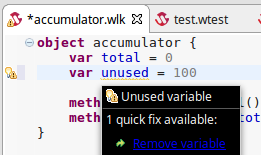
\includegraphics[scale=0.5]{images/wollok-paper-check-unusedVariable.png}
    \caption{Detection of unused variables}
    \label{fig:check-unusedVariable.png}
\end{figure}

\subsection{Type Inference}
% Type inferer
Another distinctive characteristic of the Wollok project is the type inferer.
We think that type inference is key to a simple programming environment.
On one side, it allows to detect lots of common mistakes \emph{before running the program}:
if an object does understand a message, if a wrong argument is passed, if incompatible types are mixed or even miss-spellings.
In environments without this capability it takes more time to detect errors.
Moreover, it is not uncommon that a type mistake produces a runtime error in a place different from where the mistake was done, producing confusion.

Still, providing a type inferer for a language such as Wollok has many subtleties, which deserves an independent study \cite{passerini_nicolas_extensible_2014}.
On one side we require it to be able to work without type annotations and at the same time provide feedback useful for an inexperienced programmer.
On the other side, the type system is rather complex;
for example, the presence of stand-alone objects requires the type system to handle \emph{structural types}, since a named type system would not allow them to be treated polymorphically.
Also, we want to be able to treat polymorphically stand alone objects with class-based objects.
\figref{check-messageSending.png} shows an error detected by the type inferer and how it shows the information to the programmer.
Notice that the inferred type for the object \code{ufo} is a structural type: \code{fly}

\begin{figure}[ht]
    \centering
	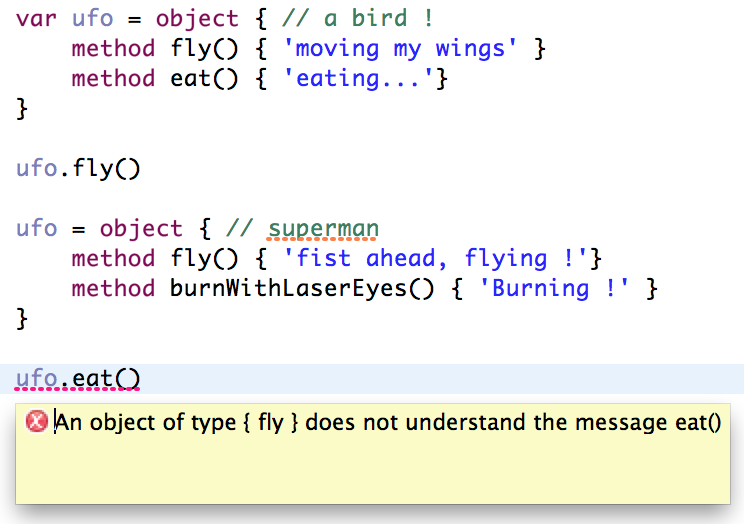
\includegraphics[scale=0.5]{images/wollok-paper-check-messageSending.png}
    \caption{Type system in action, detecting not defined method for the message sent}
    \label{fig:check-messageSending.png}
\end{figure}

\subsection{Beyond showing mistakes}
The IDE is not restricted to showing what is wrong, but also generates proposals known as \emph{quick fixes}.
\figref{quickfix.png} shows an example of one of such proposals. 
In this case the IDE detects that we are sending a message that the receiver does not understand and proposes to create the corresponding method.

\begin{figure}[ht]
    \centering
	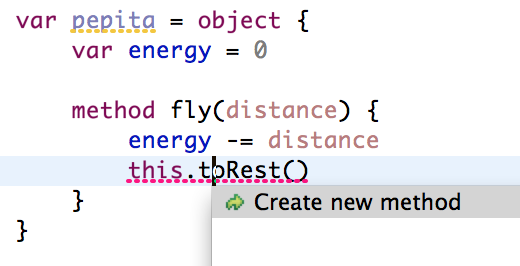
\includegraphics[scale=0.5]{images/wollok-paper-quickfix.png}
    \caption{Quick fix tool for common errors and mistakes}
    \label{fig:quickfix.png}
\end{figure}

All these tools allow the student to gain more control of his code, keeping him away from feeling lost, 
which is otherwise a common situation for a student walking his first steps into programming.
In this way the IDE becomes useful in the objective of teaching programming concepts, instead of only showing syntax errors.

